\section{Regulator PI bez odsprzęgania}
\indent Regulator PI z odsprzęganiem radzi sobie zadowalająco na zadanych przebiegach. Widać ewidentny wpływ zmiany wartości zadanej jednego wyjścia na wyjście drugie.

\subsection{Dobrane nastawy regulatora PI}
\indent Dobieranie nastaw regulatora PI zostało wykonane metodą heurystyczną, kierując się charakterystykami otrzymanych sygnałów sterowania i wyjściowych oraz również dążąc do minimalizacji błędów kwadratowych, tak by osiągnąć kompromis pomiędzy tymi wskaźnikami \\
\indent Wskaźnik jakości był wyliczany w następujący sposób dla przykładowych trajektorii zadanych:
\begin{lstlisting}[language=Matlab]
    e=rVector(ct,:) - y; % wartosc zadana- wyjscie
    errorH=e(1)^2;  
    errorT=e(2)^2;        
\end{lstlisting}

\indent Na regulator nałożono także następujące ograniczenia na minimalną i maksymalną wartość sterowania taką samą dla obu regulatorów:\\
$U_min=0$  $U_max=300$ \\

\indent W regulatorze działa także mechanizm anti windup zaczerpnięty z \href {https://www.mathworks.com/matlabcentral/answers/642205-how-do-i-set-the-saturation-output-for-pid-objects-in-matlab}{link}


\indent Dobrane parametry są następujące: \\
$KpFh=0.9$   $KiFh=0.01$ \\
$KpFcin= -0.2$  $ KiFcin2=-0.002$ \\

\subsection{PI dla przykładowych przebiegów z obiektem nielinowym}
\indent Na poniższych wykresach zostały przedstawione przykładowe przebiegi dla różnych wartości zadanych. Wyliczane wartości sterowania były podawana na model nieliniowy obiektu. \\
\indent Można zaobserwować, że zmiana jednej wartości zadanej dla jednego wyjścia wpływa na wyjście drugie. Spowodowane jest to głównie opóźnieniami w obiekcie, które sprawiają, ż regulator potrzebuje czasu aby się dostosować. \\
\indent Widać też, że regulator sobie nie radzi dla przypadku gdy temperatura zadana jest bliska temperaturze zimnej wody. Występuje wtedy uchyb na temperaturze, zaś wysokość cieczy rośnie. Pokazuje to ograniczenia regulatora oraz to, że zadawanie wartości skrajnych lub poza zakresem pracy może być niebezpieczne dla obiektu, gdy regulator ma jedne człony o większej wadze od innych. Tutaj przyczyną będzie całkowanie uchybu temperatury i zwiększanie dopływu zimnej wody oraz fakt, że cały czas jest dopływ zakłócenia o temperaturze wyższej niż temperatura zimnej wody.Czyli nie jest możliwe osiągnięcie zadanej temperatury, jednak regulator ciągle próbuje ją osiągnąć. Z tego powodu w realnym zastosowaniu należałoby podać zakres możliwych wartości zadanych, gdyż błąd operatora, wynikający z braku świadomości wpływu zakłócenia, może zniszczyć układ. 

\FloatBarrier
    \begin{figure}[h!]
   \centering
   \begin{subfigure}[b]{0.4\textwidth}
      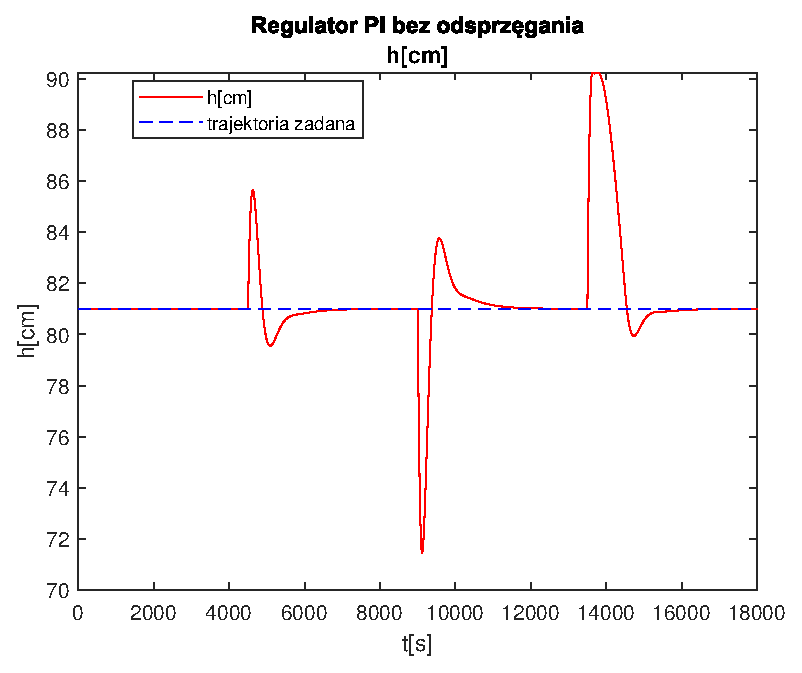
\includegraphics[width=1\linewidth]{img/PI/noDecoupler/disturbance/PINoDecouplerH2DisttrueLinfalse.eps}
      \caption{}
      \label{fig:fig:PIDecoupler2DisttrueLinfalse1}
   \end{subfigure}
       
   \begin{subfigure}[b]{0.4\textwidth}
      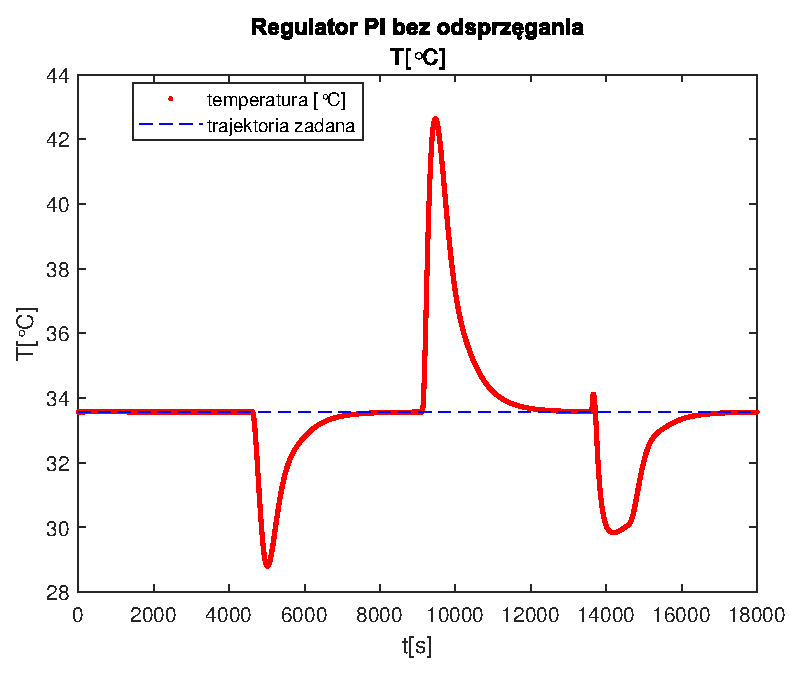
\includegraphics[width=1\linewidth]{img/PI/noDecoupler/disturbance/PINoDecouplerT2DisttrueLinfalse.eps}
      \caption{}
      \label{fig:fig:PIDecoupler2DisttrueLinfalse2}
   \end{subfigure}
       
   \begin{subfigure}[b]{0.4\textwidth}
      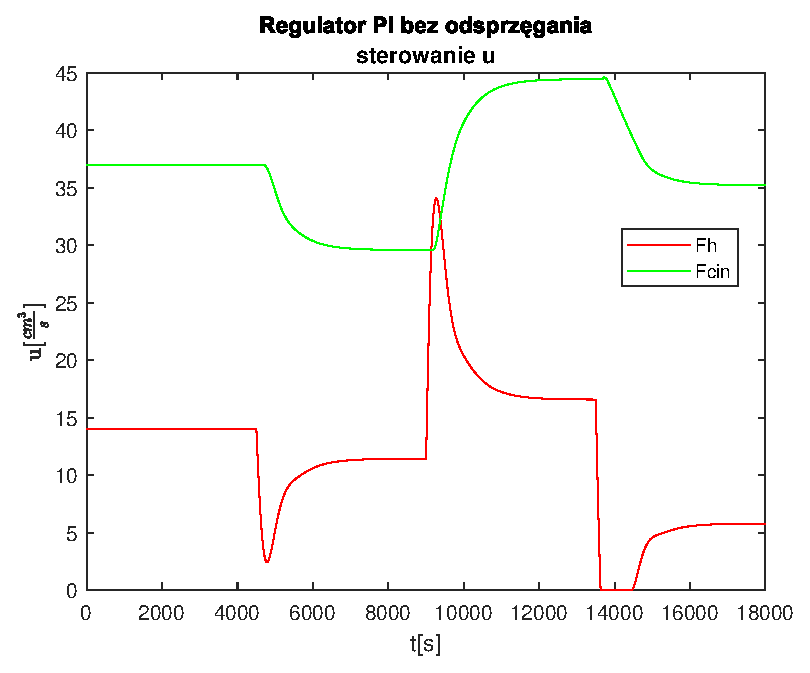
\includegraphics[width=1\linewidth]{img/PI/noDecoupler/disturbance/PINoDecouplerControl2DisttrueLinfalse.eps}
      \caption{}
      \label{fig:fig:PIDecoupler2DisttrueLinfalse3}
   \end{subfigure}
       
   \begin{subfigure}[b]{0.4\textwidth}
      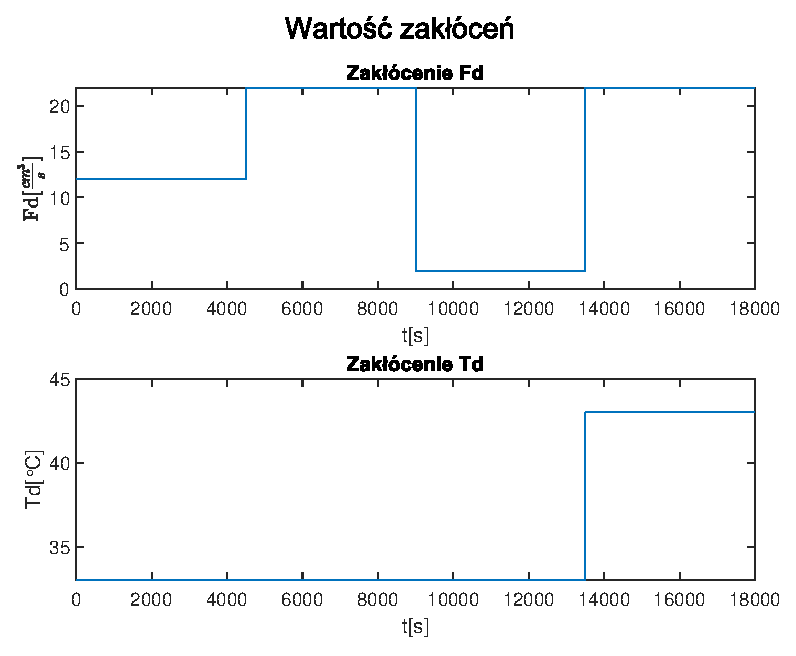
\includegraphics[width=1\linewidth]{img/PI/noDecoupler/disturbance/PIDecouplerDisturbance2DisttrueLinfalse.eps}
      \caption{}
      \label{fig:fig:PIDecoupler2DisttrueLinfalse4}
   \end{subfigure}
       
   \caption{Wykresy dla regulatora PI bez odsprzegania dla różnych wartości zakłóceń}
   \label{fig:PIDecoupler2DisttrueLinfalse}
\end{figure}
           
\begin{figure}[h!]
   \centering
   \begin{subfigure}[b]{0.4\textwidth}
      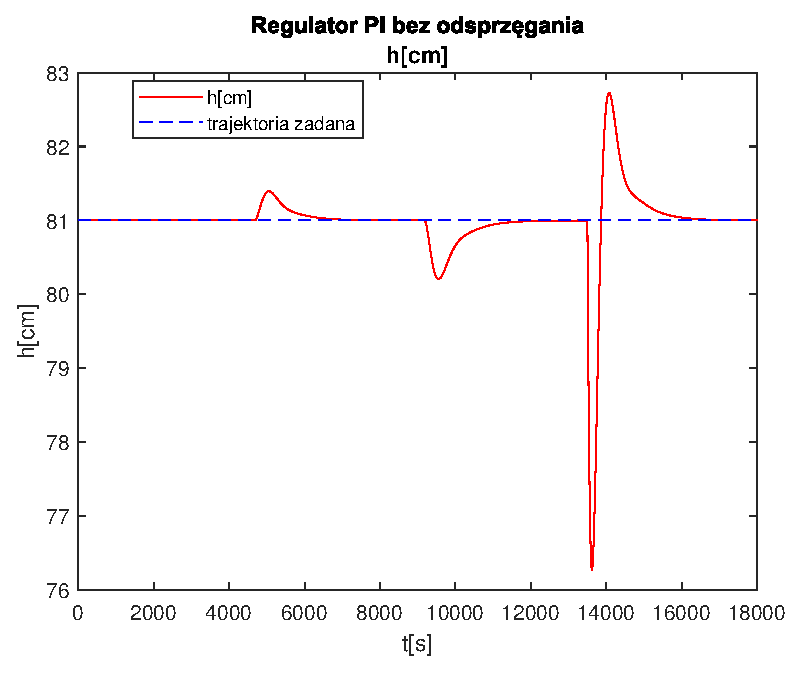
\includegraphics[width=1\linewidth]{img/PI/noDecoupler/disturbance/PINoDecouplerH3DisttrueLinfalse.eps}
      \caption{}
      \label{fig:fig:PIDecoupler3DisttrueLinfalse1}
   \end{subfigure}
       
   \begin{subfigure}[b]{0.4\textwidth}
      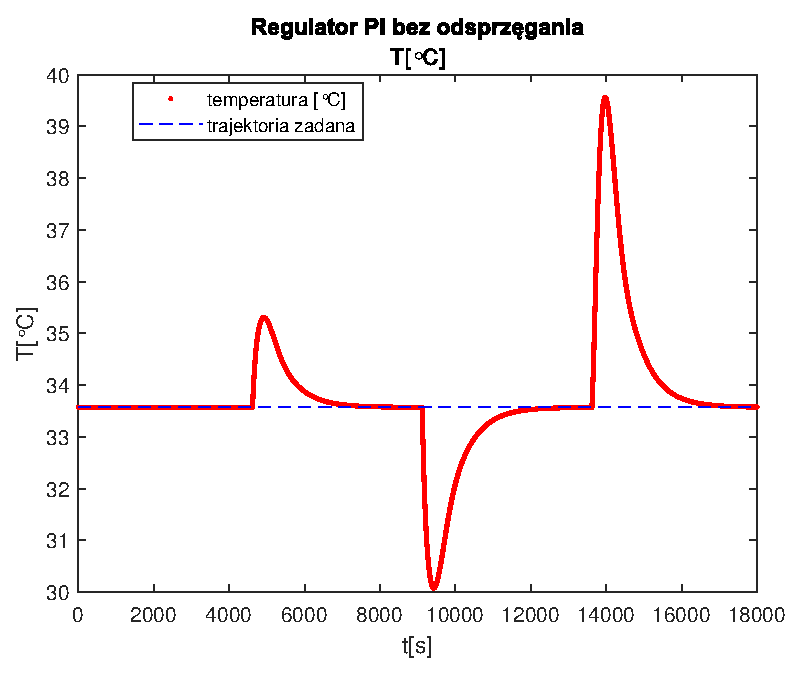
\includegraphics[width=1\linewidth]{img/PI/noDecoupler/disturbance/PINoDecouplerT3DisttrueLinfalse.eps}
      \caption{}
      \label{fig:fig:PIDecoupler3DisttrueLinfalse2}
   \end{subfigure}
       
   \begin{subfigure}[b]{0.4\textwidth}
      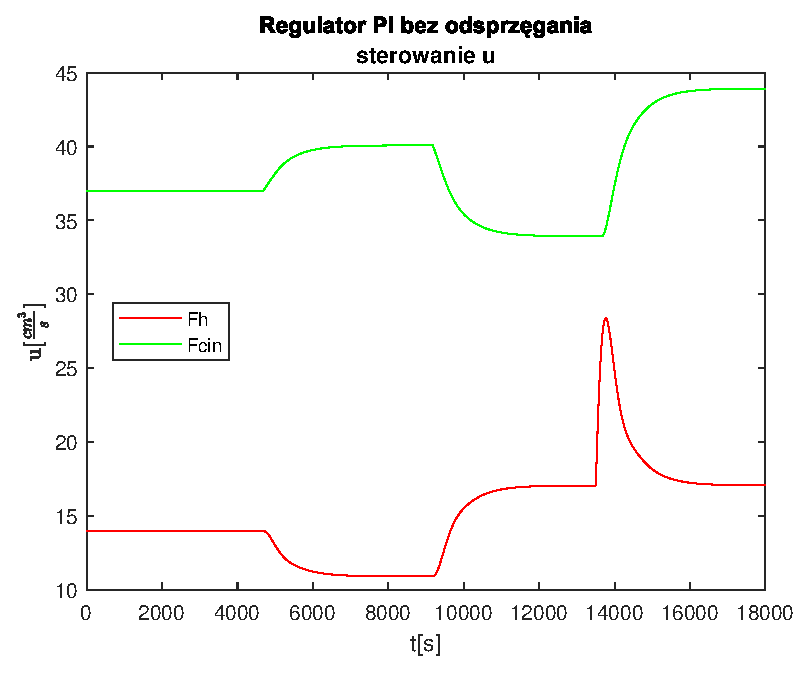
\includegraphics[width=1\linewidth]{img/PI/noDecoupler/disturbance/PINoDecouplerControl3DisttrueLinfalse.eps}
      \caption{}
      \label{fig:fig:PIDecoupler3DisttrueLinfalse3}
   \end{subfigure}
       
   \begin{subfigure}[b]{0.4\textwidth}
      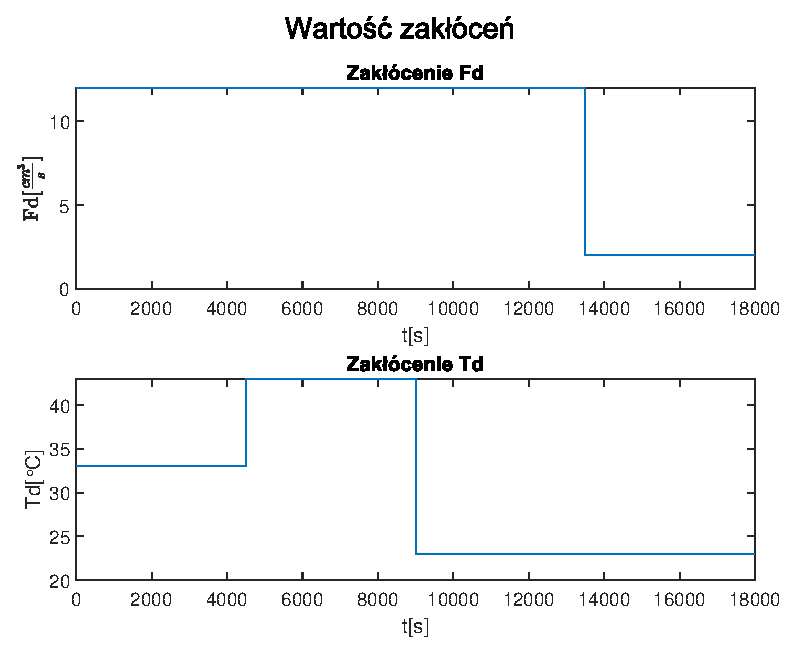
\includegraphics[width=1\linewidth]{img/PI/noDecoupler/disturbance/PIDecouplerDisturbance3DisttrueLinfalse.eps}
      \caption{}
      \label{fig:fig:PIDecoupler3DisttrueLinfalse4}
   \end{subfigure}
       
   \caption{Wykresy dla regulatora PI bez odsprzegania dla różnych wartości zakłóceń}
   \label{fig:PIDecoupler3DisttrueLinfalse}
\end{figure}
           

\FloatBarrier


\subsection{PI dla przykładowych przebiegów z obiektem zlinearyzowanym}
\indent Badając jak zachowa się regulator po symulacji na obiekcie zlinearyzowanym widać, że zachowuje się on trochę bardziej stabilnie w wartości skrajnej temperatury zadanej. Jest to zachowanie niebezpieczne, ponieważ wynik z symulacji nie ma przełożenia na rzeczywisty obiekt. Czyli w tym wypadku jest pokazane, że zadana temperaturę można osiągnąć, gdy w rzeczywistości nie jest to możliwe. Należy zatem mieć to na uwadze ograniczenia wynikające z możliwości modelu liniowego.
\FloatBarrier
    \begin{figure}[h!]
   \centering
   \begin{subfigure}[b]{0.4\textwidth}
      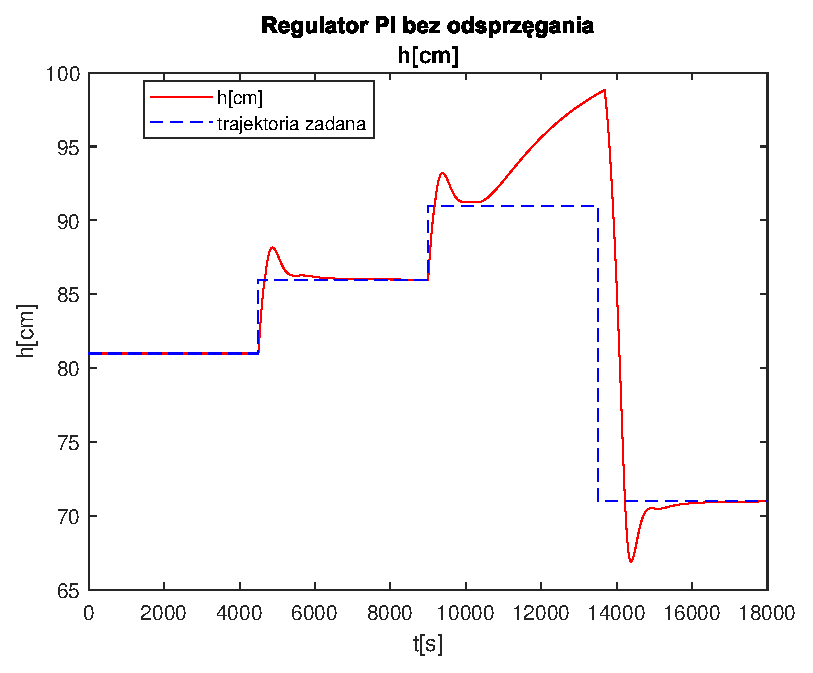
\includegraphics[width=1\linewidth]{img/PI/noDecoupler/noDisturbance/PINoDecouplerH1Lintrue.eps}
      \caption{}
      \label{fig:fig:PINodDecoupler1Lintrue1}
   \end{subfigure}
       
   \begin{subfigure}[b]{0.4\textwidth}
      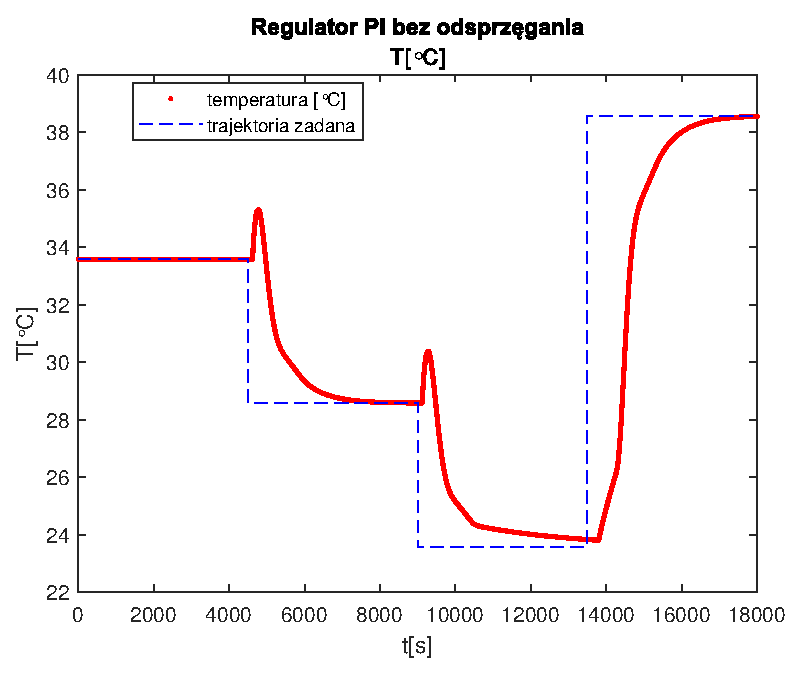
\includegraphics[width=1\linewidth]{img/PI/noDecoupler/noDisturbance/PINoDecouplerT1Lintrue.eps}
      \caption{}
      \label{fig:fig:PINodDecoupler1Lintrue2}
   \end{subfigure}
       
   \begin{subfigure}[b]{0.4\textwidth}
      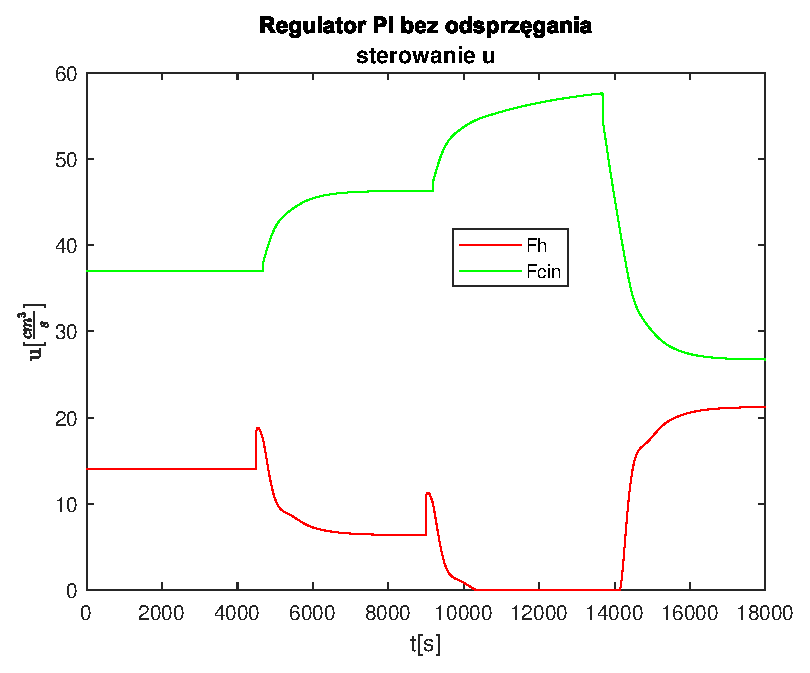
\includegraphics[width=1\linewidth]{img/PI/noDecoupler/noDisturbance/PINoDecouplerControl1Lintrue.eps}
      \caption{}
      \label{fig:fig:PINodDecoupler1Lintrue3}
   \end{subfigure}
       
   \caption{Wykresy dla regulatora PI bez odsprzegania.}
   \label{fig:PINodDecoupler1Lintrue}
\end{figure}
           
\begin{figure}[h!]
   \centering
   \begin{subfigure}[b]{0.4\textwidth}
      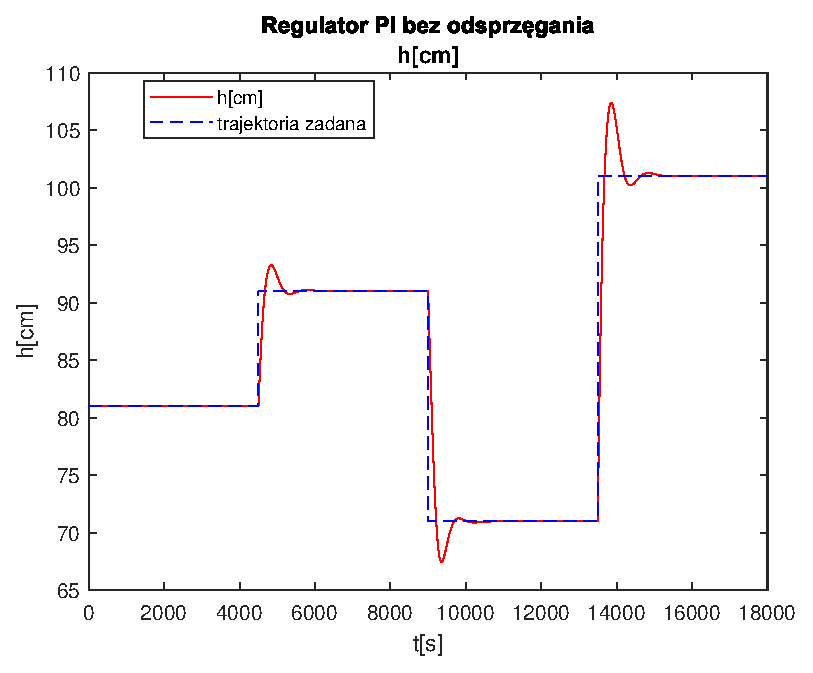
\includegraphics[width=1\linewidth]{img/PI/noDecoupler/noDisturbance/PINoDecouplerH2Lintrue.eps}
      \caption{}
      \label{fig:fig:PINodDecoupler2Lintrue1}
   \end{subfigure}
       
   \begin{subfigure}[b]{0.4\textwidth}
      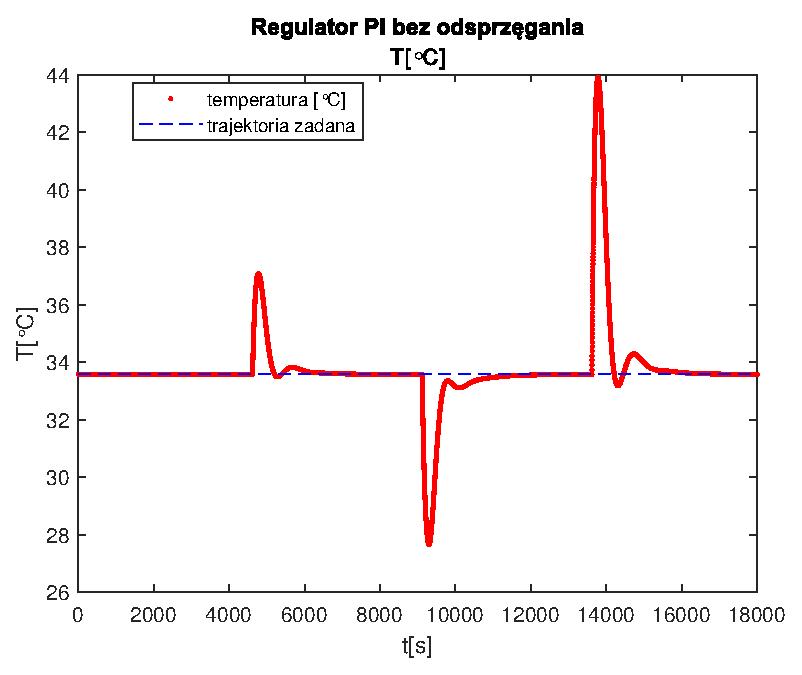
\includegraphics[width=1\linewidth]{img/PI/noDecoupler/noDisturbance/PINoDecouplerT2Lintrue.eps}
      \caption{}
      \label{fig:fig:PINodDecoupler2Lintrue2}
   \end{subfigure}
       
   \begin{subfigure}[b]{0.4\textwidth}
      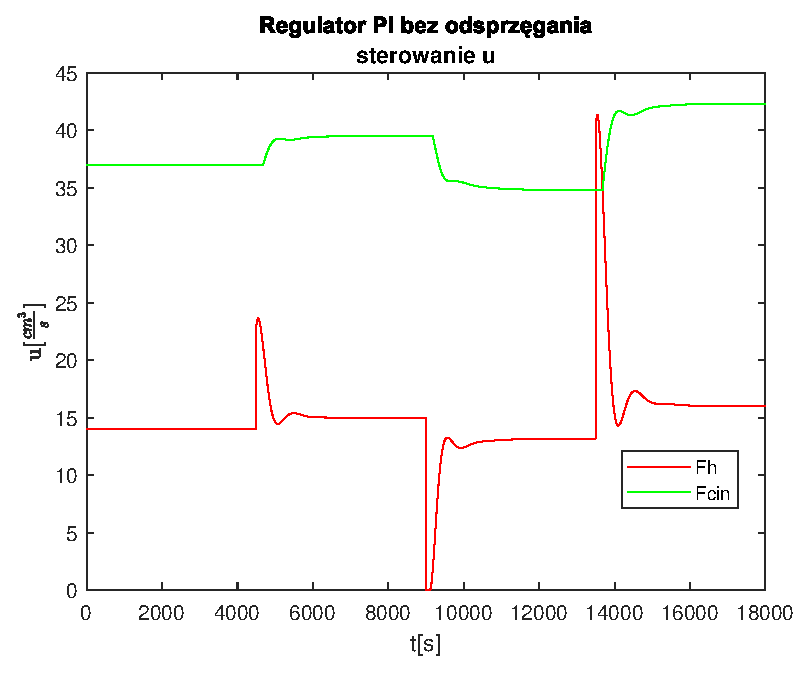
\includegraphics[width=1\linewidth]{img/PI/noDecoupler/noDisturbance/PINoDecouplerControl2Lintrue.eps}
      \caption{}
      \label{fig:fig:PINodDecoupler2Lintrue3}
   \end{subfigure}
       
   \caption{Wykresy dla regulatora PI bez odsprzegania.}
   \label{fig:PINodDecoupler2Lintrue}
\end{figure}
           
\begin{figure}[h!]
   \centering
   \begin{subfigure}[b]{0.4\textwidth}
      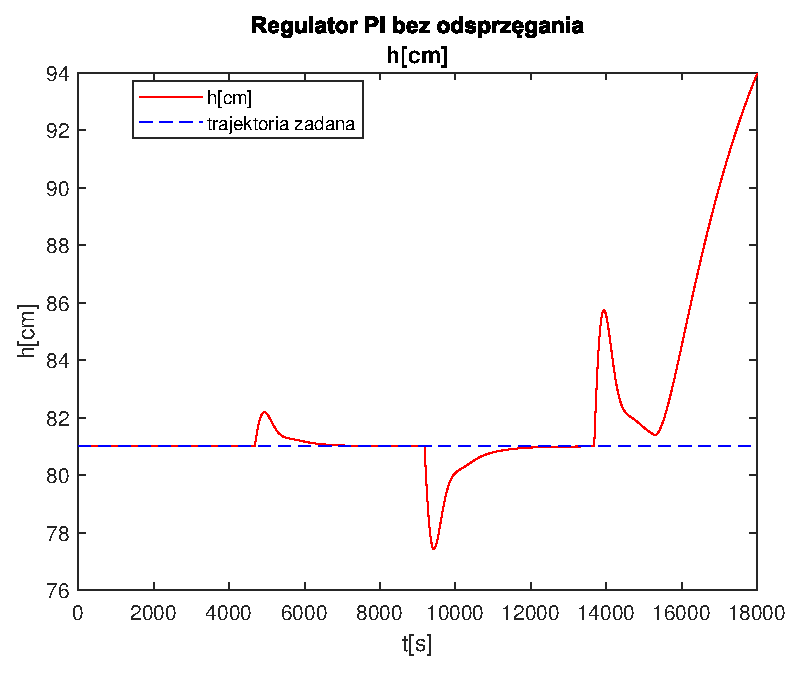
\includegraphics[width=1\linewidth]{img/PI/noDecoupler/noDisturbance/PINoDecouplerH3Lintrue.eps}
      \caption{}
      \label{fig:fig:PINodDecoupler3Lintrue1}
   \end{subfigure}
       
   \begin{subfigure}[b]{0.4\textwidth}
      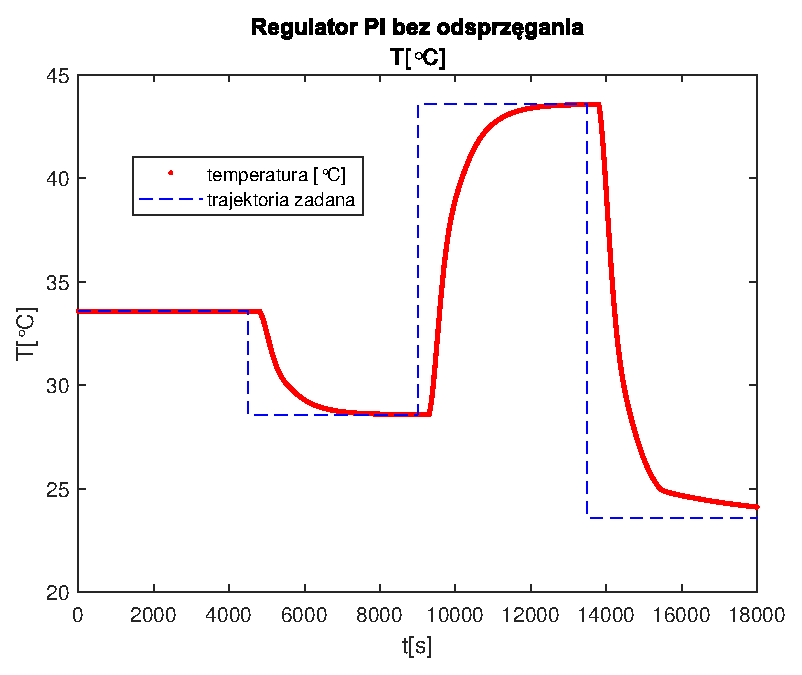
\includegraphics[width=1\linewidth]{img/PI/noDecoupler/noDisturbance/PINoDecouplerT3Lintrue.eps}
      \caption{}
      \label{fig:fig:PINodDecoupler3Lintrue2}
   \end{subfigure}
       
   \begin{subfigure}[b]{0.4\textwidth}
      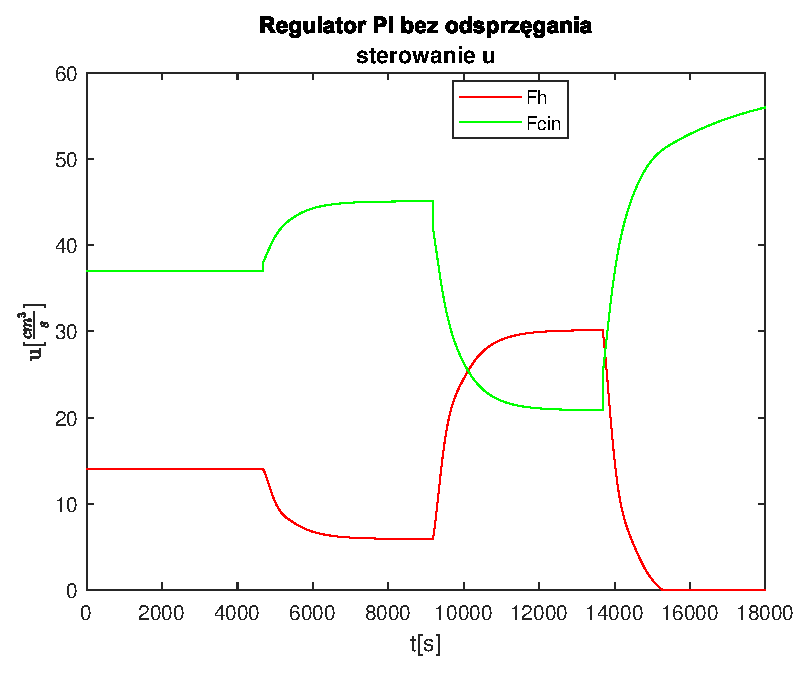
\includegraphics[width=1\linewidth]{img/PI/noDecoupler/noDisturbance/PINoDecouplerControl3Lintrue.eps}
      \caption{}
      \label{fig:fig:PINodDecoupler3Lintrue3}
   \end{subfigure}
       
   \caption{Wykresy dla regulatora PI bez odsprzegania.}
   \label{fig:PINodDecoupler3Lintrue}
\end{figure}
           

\FloatBarrier

\subsection{PI ze zmianą zakłócenia z obiektem nielinowym}
\indent Z wykresów zaprezentowanych w tej sekcji można zaobserwować, że regulator radzi sobie dobrze ze zmianą zakłócenia. Na początku wyjścia odbiegają od wartości zadanych, nie są to jednak są duże wartości. Regulator jest w stanie szybko skompensować zakłócenie i działać potem poprawnie.
\FloatBarrier
    \begin{figure}[h!]
   \centering
   \begin{subfigure}[b]{0.4\textwidth}
      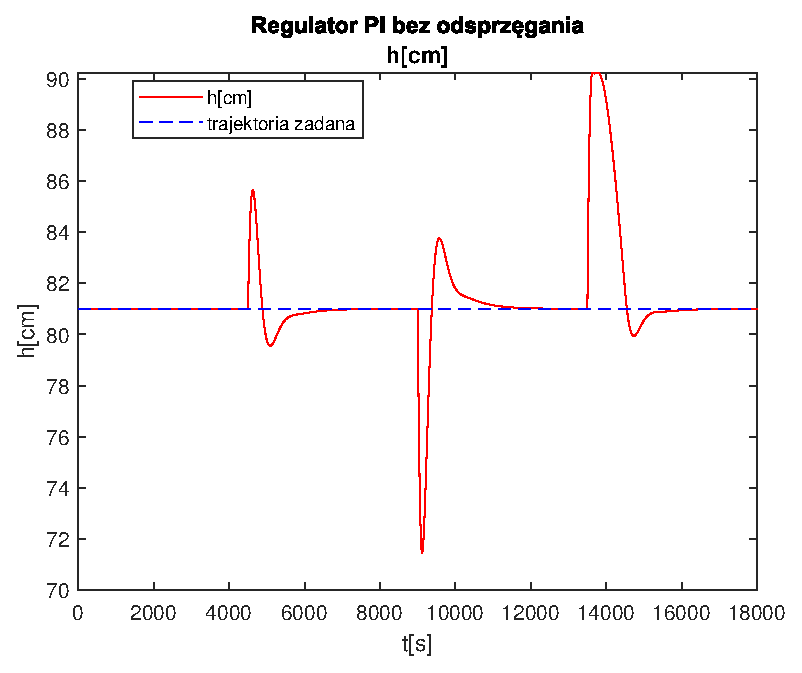
\includegraphics[width=1\linewidth]{img/PI/noDecoupler/disturbance/PINoDecouplerH2DisttrueLinfalse.eps}
      \caption{}
      \label{fig:fig:PIDecoupler2DisttrueLinfalse1}
   \end{subfigure}
       
   \begin{subfigure}[b]{0.4\textwidth}
      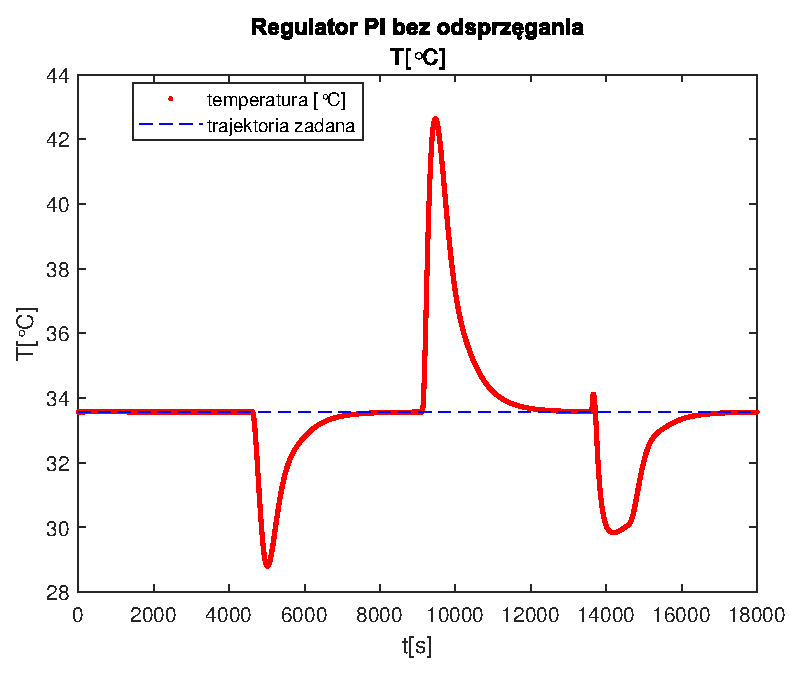
\includegraphics[width=1\linewidth]{img/PI/noDecoupler/disturbance/PINoDecouplerT2DisttrueLinfalse.eps}
      \caption{}
      \label{fig:fig:PIDecoupler2DisttrueLinfalse2}
   \end{subfigure}
       
   \begin{subfigure}[b]{0.4\textwidth}
      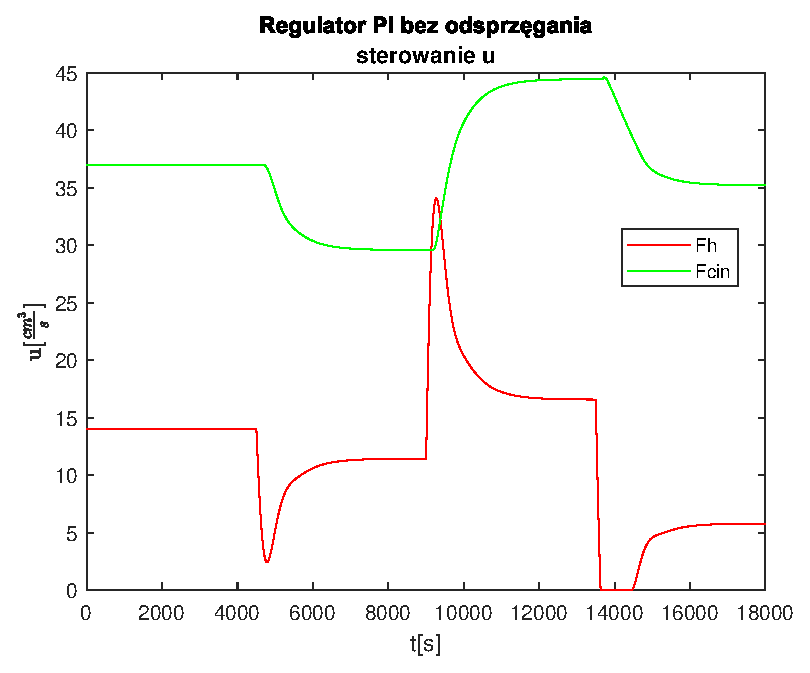
\includegraphics[width=1\linewidth]{img/PI/noDecoupler/disturbance/PINoDecouplerControl2DisttrueLinfalse.eps}
      \caption{}
      \label{fig:fig:PIDecoupler2DisttrueLinfalse3}
   \end{subfigure}
       
   \begin{subfigure}[b]{0.4\textwidth}
      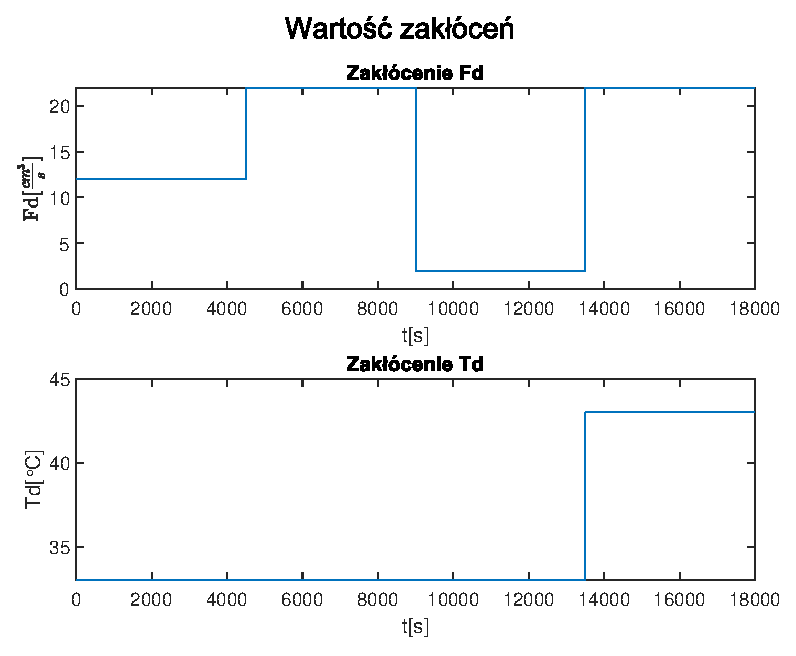
\includegraphics[width=1\linewidth]{img/PI/noDecoupler/disturbance/PIDecouplerDisturbance2DisttrueLinfalse.eps}
      \caption{}
      \label{fig:fig:PIDecoupler2DisttrueLinfalse4}
   \end{subfigure}
       
   \caption{Wykresy dla regulatora PI bez odsprzegania dla różnych wartości zakłóceń}
   \label{fig:PIDecoupler2DisttrueLinfalse}
\end{figure}
           
\begin{figure}[h!]
   \centering
   \begin{subfigure}[b]{0.4\textwidth}
      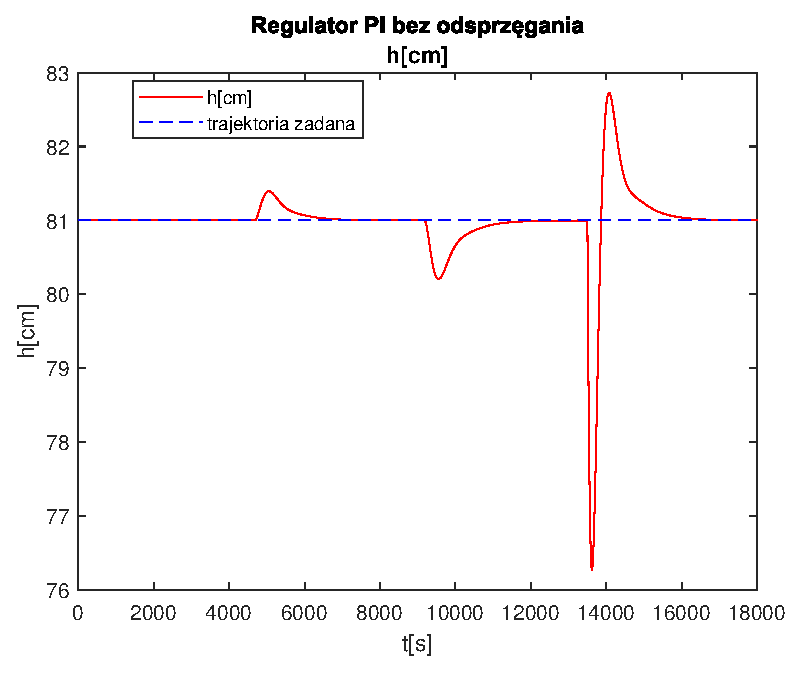
\includegraphics[width=1\linewidth]{img/PI/noDecoupler/disturbance/PINoDecouplerH3DisttrueLinfalse.eps}
      \caption{}
      \label{fig:fig:PIDecoupler3DisttrueLinfalse1}
   \end{subfigure}
       
   \begin{subfigure}[b]{0.4\textwidth}
      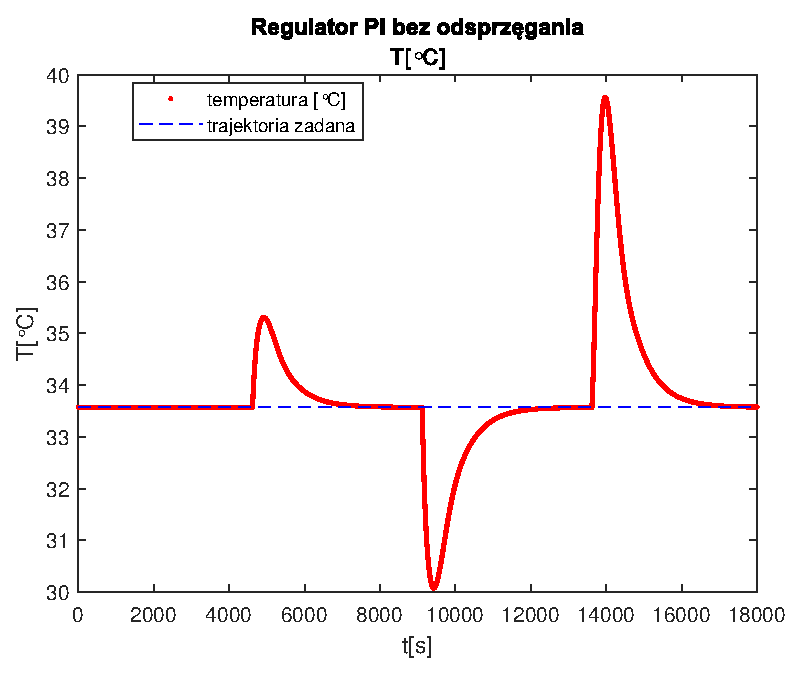
\includegraphics[width=1\linewidth]{img/PI/noDecoupler/disturbance/PINoDecouplerT3DisttrueLinfalse.eps}
      \caption{}
      \label{fig:fig:PIDecoupler3DisttrueLinfalse2}
   \end{subfigure}
       
   \begin{subfigure}[b]{0.4\textwidth}
      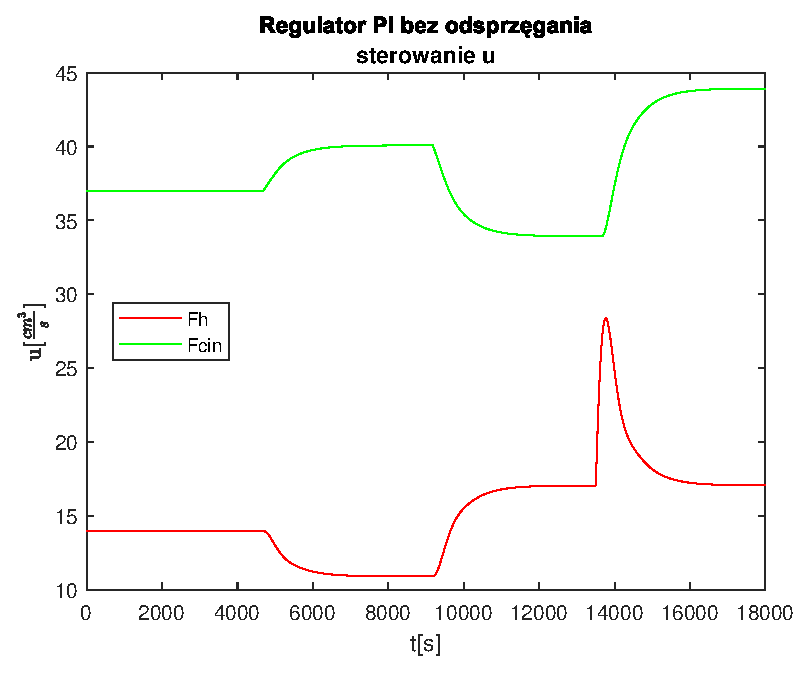
\includegraphics[width=1\linewidth]{img/PI/noDecoupler/disturbance/PINoDecouplerControl3DisttrueLinfalse.eps}
      \caption{}
      \label{fig:fig:PIDecoupler3DisttrueLinfalse3}
   \end{subfigure}
       
   \begin{subfigure}[b]{0.4\textwidth}
      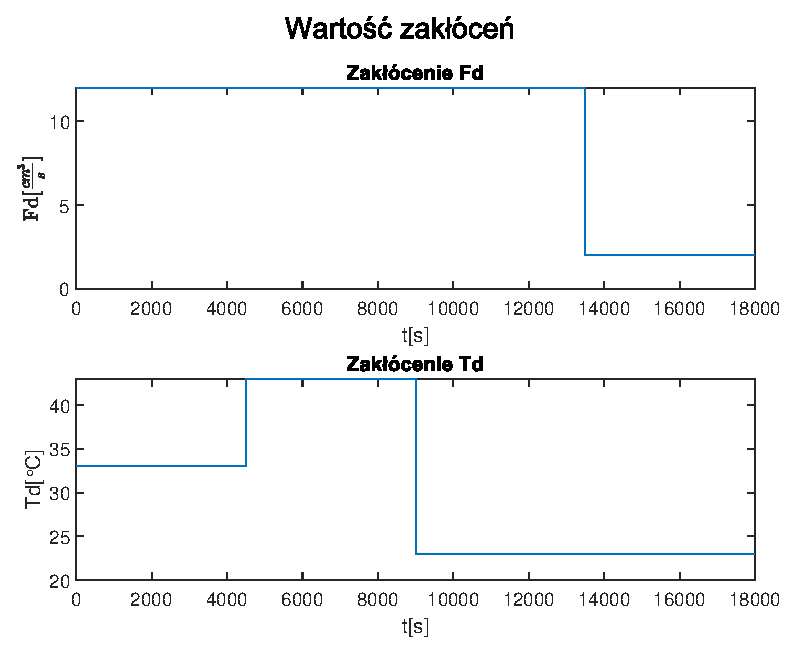
\includegraphics[width=1\linewidth]{img/PI/noDecoupler/disturbance/PIDecouplerDisturbance3DisttrueLinfalse.eps}
      \caption{}
      \label{fig:fig:PIDecoupler3DisttrueLinfalse4}
   \end{subfigure}
       
   \caption{Wykresy dla regulatora PI bez odsprzegania dla różnych wartości zakłóceń}
   \label{fig:PIDecoupler3DisttrueLinfalse}
\end{figure}
           

\FloatBarrier


\subsection{Napełniania zbiornika do punktu pracy PI z modelem nieliniowym}
\indent W ramach testów zostało sprawdzone jak regulator radzi sobie z zapełnianiem zbiornika. W związku z tym, że sterownie dojścia zimnej wody jest opóźnione występuje znaczące przergulowanie temperatury, ponieważ głównie to regulator odpowiadający za dopływ ciepłej wody odpowiada za strumień wejściowy. Dzieje się tak ponieważ temperatura zadana jest wyższa niż obecna w zbiorniku oraz że zimna woda działa z opóźnieniem. Po chwili gdy wejście zimnej wody również zaczyna mieć wpływ w obiekcie układ się stabilizuje.
\FloatBarrier
    \begin{figure}[h!]
   \centering
   \begin{subfigure}[b]{0.4\textwidth}
      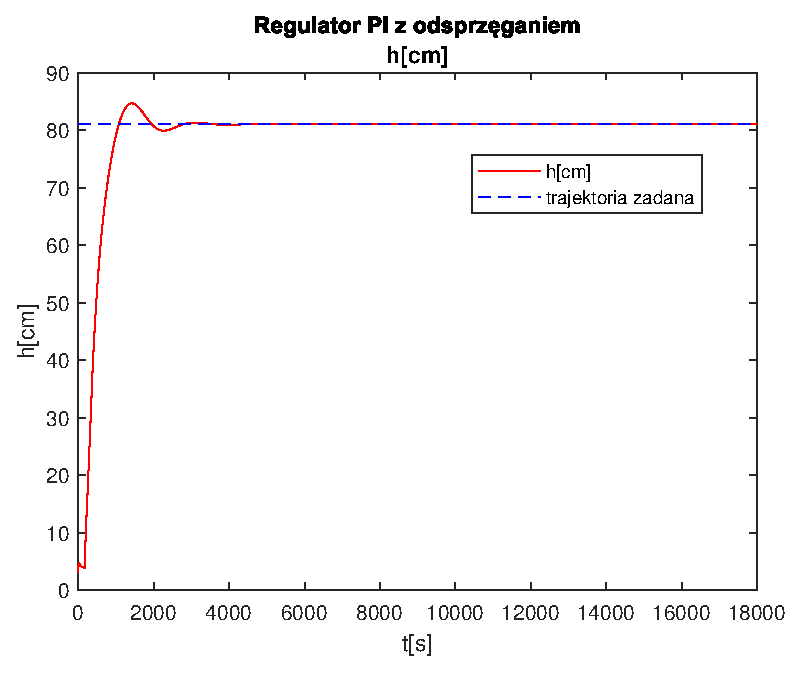
\includegraphics[width=1\linewidth]{img/PI/decoupler/noDisturbance/PIDecouplerH0.eps}
      \caption{}
      \label{fig:fig:PIDecoupler01}
   \end{subfigure}
       
   \begin{subfigure}[b]{0.4\textwidth}
      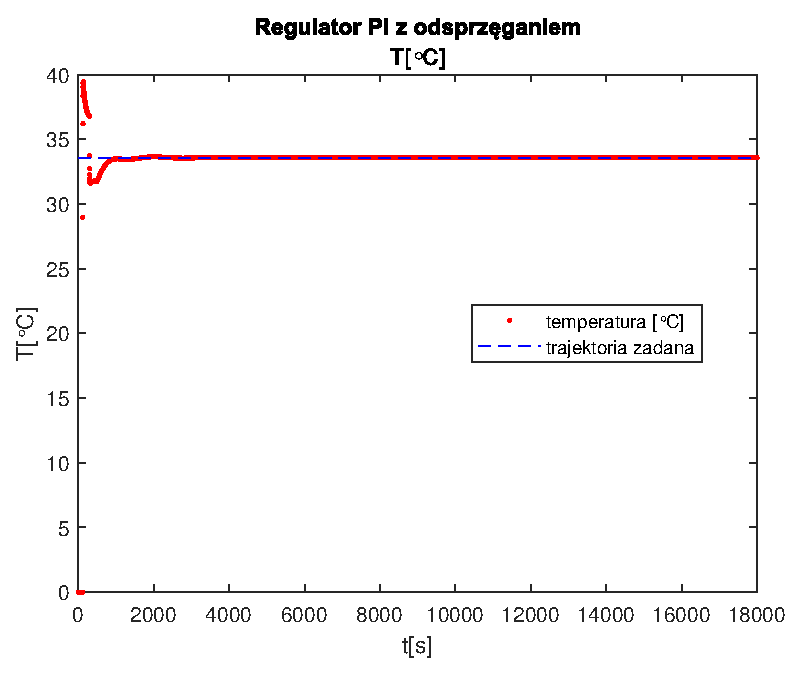
\includegraphics[width=1\linewidth]{img/PI/decoupler/noDisturbance/PIDecouplerT0.eps}
      \caption{}
      \label{fig:fig:PIDecoupler02}
   \end{subfigure}
       
   \begin{subfigure}[b]{0.4\textwidth}
      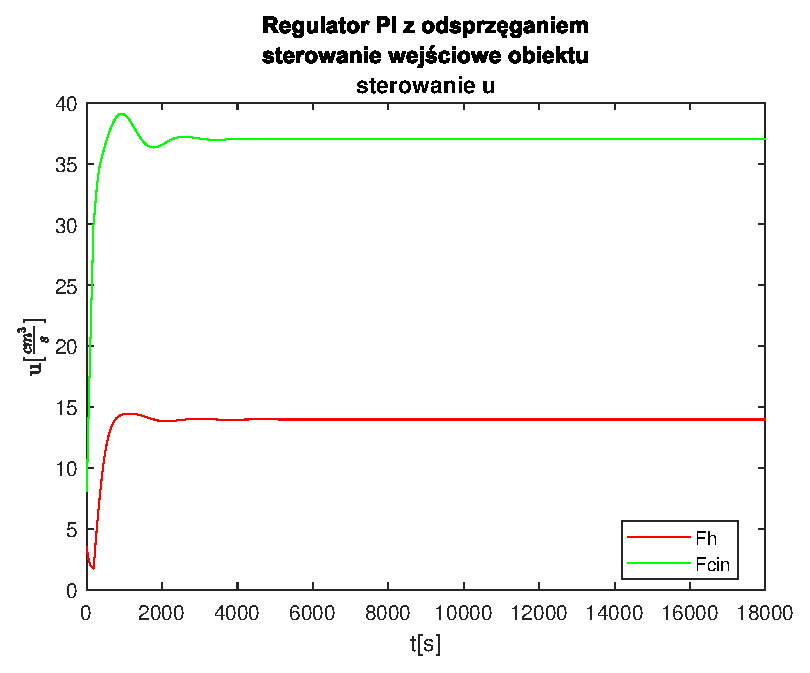
\includegraphics[width=1\linewidth]{img/PI/decoupler/noDisturbance/PIDecouplerControl0.eps}
      \caption{}
      \label{fig:fig:PIDecoupler03}
   \end{subfigure}
       
   \begin{subfigure}[b]{0.4\textwidth}
      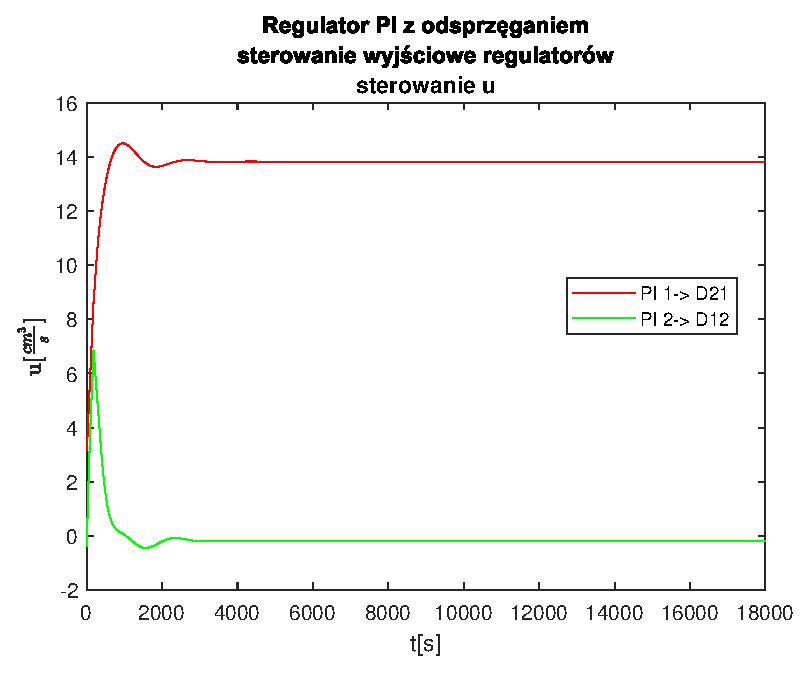
\includegraphics[width=1\linewidth]{img/PI/decoupler/noDisturbance/PIDecouplerControlD0.eps}
      \caption{}
      \label{fig:fig:PIDecoupler04}
   \end{subfigure}
       
   \caption{Wykresy dla regulatora PI z odsprzeganiem.}
   \label{fig:PIDecoupler0}
\end{figure}
           

\FloatBarrier 